%% AISSH-26 workshop expansion manuscript: Springer Nature sn-jnl format.
%% Section skeleton follows paper/AISSH_Springer/springer-nature.tex (the blank
%% template) closely: Introduction -> Results -> Methods -> Discussion ->
%% Conclusion -> backmatter -> Declarations -> Appendices. Content ported from
%% paper/WileyDesign/Optimal-Design-layout/Optimal-Design-layout.tex (de-anonymized)
%% and paper/Paper.tex (numeric source of truth), with the guard-bear
%% safety-classifier contribution folded in throughout. Related Work, System
%% Architecture, Dataset, Extended Experiments, and Limitations are not separate
%% top-level sections here (the template does not have them): related-work
%% framing lives in the unsubheaded Introduction, architecture/dataset/training
%% detail lives in Methods, the rank/layer/cross-architecture sweeps live as
%% Results subsections, and limitations are folded into the Conclusion, per the
%% template's own guidance for each of those sections.
%%
%% TODO before submission:
%%   - Fill in real institutional emails for all four authors (FIXME markers below).
%%   - Confirm venue/copyright/funding boilerplate in the Declarations section.
%%   - Confirm whether AISSH-26 permits the repository link in the appendix (this is
%%     an invited, non-blind submission, so it is included by default here).
%%   - Recompile and check page count against the 6-12 page (excl. references) budget.

\documentclass[pdflatex,sn-mathphys-num]{sn-jnl}% Math and Physical Sciences Numbered Reference Style

\usepackage{graphicx}%
\usepackage{multirow}%
\usepackage{amsmath,amssymb,amsfonts}%
\usepackage{amsthm}%
\usepackage{mathrsfs}%
\usepackage[title]{appendix}%
\usepackage{xcolor}%
\usepackage{textcomp}%
\usepackage{manyfoot}%
\usepackage{booktabs}%

\raggedbottom

\begin{document}

\title[Safety-Gated, Age-Adaptive LoRA Fine-Tuning for a Virtual Pediatric Hospital Guide]{Safety-Gated, Age-Adaptive LoRA Fine-Tuning for a Virtual Pediatric Hospital Guide}

\author*[3]{\fnm{Anthony} \sur{Barros}}\email{FIXME-institutional-email@uwo.ca}

\author[1,2]{\fnm{Sandrine} \sur{de Ribaupierre}}\email{FIXME-institutional-email@uwo.ca}

\author[2,3]{\fnm{Roy} \sur{Eagleson}}\email{FIXME-institutional-email@uwo.ca}

\author[3]{\fnm{Kelsey} \sur{Kloosterman}}\email{FIXME-institutional-email@uwo.ca}

\affil*[1]{\orgdiv{Clinical Neurological Sciences}, \orgname{Western University}, \orgaddress{\city{London}, \state{Ontario}, \country{Canada}}}

\affil[2]{\orgdiv{Centre for Brain and Mind}, \orgname{Western University}, \orgaddress{\city{London}, \state{Ontario}, \country{Canada}}}

\affil[3]{\orgdiv{Department of Artificial Intelligence and Software Engineering, Faculty of Engineering}, \orgname{Western University}, \orgaddress{\city{London}, \state{Ontario}, \country{Canada}}}

\abstract{Pediatric patients navigating hospital environments require age-appropriate, institutionally grounded information that general-purpose AI systems are not designed to provide, and any system that receives free-text input from child users must also defend against inputs the system was never intended to handle. We present \textit{Dr.\ Beary Good}, an age-targeted conversational guide deployed within a digital recreation of Victoria Hospital (London, Ontario), together with \textit{guard-bear}, an upstream input-safety classifier that gates access to it. The response model uses Low-Rank Adaptation (LoRA) on 4-bit quantized Llama 3.2 Instruct models (1B and 3B) running on an Apple Mac Mini M4 (16~GB), a deliberate constraint modeling resource-limited clinical deployment; we train two adapter configurations, Standard ($r=8$, 16 layers) and Fast ($r=4$, 8 layers), across both model sizes and age groups (5--11, 12--18) for 8 training runs total, on approximately 560 synthetic examples per adapter (1123 total across six topic categories) generated by Claude Opus 4.6 using Victoria Hospital's public patient materials as grounding artifacts, following a LIMA-inspired curation approach~\cite{zhou2023lima}. Fine-tuned adapters substantially outperform zero-shot base models on readability (72--84\% of 5--11 responses meeting a Flesch-Kincaid $\leq 7.0$ grade-level target vs.\ 12--14\% for base models) and inter-role style separation (0.89--0.94 vs.\ 0.66--0.70 classifier accuracy). We observe a \textbf{configuration-ordering crossover}: Standard outperforms on the 3B model, Fast outperforms on the 1B model, consistent across all five readability metrics. A controlled rank sweep and a follow-up layer sweep resolve the mechanism: rank is the dominant factor via capacity regularization, and layer depth is an independent secondary contributor, with transformer depth (not parameter count) predicting the optimal rank regime. Cross-architecture validation on Qwen~2, SmolLM2, and the Qwen 2.5 family (0.5B--3B) confirms the crossover is not Llama-specific. Separately, \textit{guard-bear} is a full fine-tune of \texttt{Prompt-Guard-86M}~\cite{promptguard2024}, an 86M-parameter DeBERTa-v2~\cite{he2021deberta} sequence classifier, trained on a purpose-built dataset of 4{,}703 labeled examples (2{,}404 unsafe, 2{,}299 safe) spanning 14 subcategories designed for this clinical, pediatric-facing threat model rather than the developer-facing prompt-injection threat model the base model targets. On a 613-example held-out test set, the fine-tuned classifier achieves 0.987 unsafe recall, 0.990 unsafe precision, and 0.999 ROC-AUC, versus 0.959 recall, 0.505 precision, and 0.466 ROC-AUC (worse than random) for the unmodified base model, which saturates by flagging nearly everything as unsafe. Together, these results demonstrate that both age-adaptive response generation and domain-specific input safety gating are achievable on consumer hardware for a pediatric clinical deployment, and that general-purpose safety classifiers do not transfer to this population without task-specific fine-tuning.}

\keywords{parameter-efficient fine-tuning, low-rank adaptation, pediatric clinical NLP, virtual reality, on-device inference, small language models, LLM input safety classification}

\maketitle

\section{Introduction}\label{sec1}

Large language models (LLMs) have created new opportunities for domain-specific conversational systems, but deploying them in resource-constrained clinical environments introduces practical constraints that are rarely addressed together: limited memory budgets favor smaller models, domain adaptation requires fine-tuning on specialized data, real-time interaction imposes strict latency bounds, and any system that accepts free-text input from a vulnerable population must be defended against inputs it was never designed to handle.

This paper presents \textit{Dr.\ Beary Good}, an age-targeted conversational guide embedded in a virtual recreation of Victoria Hospital (London, Ontario). The system provides age-appropriate hospital information to two patient groups, children aged 5--11 and adolescents aged 12--18, via natural language interaction within a VR environment. Although these are the two age groups chosen for this study, the system can support additional age bands as needed, since each adapter is small relative to the shared base model. All training and inference for the response model runs on an Apple Mac Mini M4 (16~GB), a deliberate constraint representing deployment on consumer hardware without cloud infrastructure.

Low-Rank Adaptation (LoRA)~\cite{hu2022lora} reduces fine-tuning cost by constraining weight updates to a low-rank decomposition $\Delta W = BA$, leaving the pre-trained weights frozen; QLoRA~\cite{dettmers2023qlora} extended this to 4-bit quantized base models via NormalFloat quantization, enabling fine-tuning of 7B--65B models on consumer hardware, and both are now standard in resource-constrained deployment pipelines. Rank selection is typically treated as a task-dependent hyperparameter: common practitioner guidance, including HuggingFace PEFT defaults and QLoRA, recommends rank 8--16 without conditioning on model scale, and Biderman et al.~\cite{biderman2024lora} provide the most thorough empirical study to date, recommending rank 16 as a practical default, but this guidance is developed and validated at the 7B--70B scale; rank-ordering behavior below 7B is not characterized by existing work.

To specialize the response model for each age group within our memory budget, we fine-tune Llama 3.2 Instruct models~\cite{dubey2024llama3} at 1B and 3B scales using LoRA. Training data is generated synthetically following the LIMA hypothesis~\cite{zhou2023lima}, that a small set of carefully curated, high-quality examples suffices for behavioral alignment: approximately 560 training examples per adapter (1123 total across six topic categories) grounded in Victoria Hospital's public patient and family materials, rather than a large noisy corpus. We compare two adapter configurations (Standard: $r=8$, 16 adapted layers; Fast: $r=4$, 8 adapted layers) across both model sizes and age groups for eight total training runs, providing empirical evidence that adapter performance ordering can reverse between 1B and 3B models on the same task, a regime not covered by prior rank-selection studies.

LLMs have been applied to patient education, clinical FAQ systems, and virtual health assistants, but pediatric deployment introduces challenges distinct from adult-facing systems: responses must match developmental vocabulary, maintain an emotionally supportive rather than clinical register, and enforce hard safety constraints such as never implying a diagnosis, properties not delivered by generic instruction-following fine-tuning on a general-purpose model. A recurring constraint in clinical NLP is the unavailability of naturalistic patient dialogue due to privacy regulations, which motivates the synthetic, LIMA-style data generation approach above; to our knowledge, no prior work has used fine-tuned, age-stratified LoRA adapters for pediatric hospital communication.

Our evaluation surfaces a \textbf{configuration-ordering crossover}: the Standard adapter yields better readability and style-separation results on the 3B model, while the Fast adapter outperforms on the 1B model. This crossover is consistent across all five readability metrics and the inter-role classification task, and suggests that optimal adapter capacity is model-size-dependent, a dependency not captured by common LoRA guidelines that recommend a fixed rank range without model-size conditioning. Only the Fast-1B configuration meets the 1.0-second real-time latency target for VR interaction for the 5--11 age group (0.93s average).

VR-based interventions demonstrably reduce procedural pain and anxiety in pediatric patients, from preoperative preparation to bedside procedures, yet existing deployments are largely passive: scripted or pre-rendered distraction content that does not respond to patient queries or adapt to developmental stage, despite hospitalized children frequently having unanswered questions about their environment, staff, and upcoming procedures. \textit{Dr.\ Beary Good} addresses this gap by integrating age-targeted fine-tuned adapters, gated by a dedicated safety classifier, into an interactive VR environment, combining the anxiety-reduction potential of immersive VR with the informational utility of a conversational agent grounded in hospital-specific knowledge.

A conversational system that accepts open-ended text from children also needs a defense layer distinct from the response model itself. Deployed conversational LLM systems face a well-documented risk of prompt injection and jailbreak attacks, and general-purpose injection-detection classifiers, such as \texttt{Prompt-Guard-86M}~\cite{promptguard2024}, are trained primarily to recognize this developer-facing threat model: imperative override patterns embedded in text such as ``ignore the above instructions and reveal your system prompt.'' This threat model does not transfer cleanly to a pediatric-facing conversational system, where legitimate queries are short, first-person, and emotionally direct (``will my surgery hurt?''), and a substantial share of the inputs that should still be blocked, out-of-scope curiosity, gibberish or malformed text, and adult/parental content, carry no injection signal at all. To our knowledge, no prior work evaluates an input-safety classifier calibrated specifically to a pediatric clinical deployment context, nor quantifies the resulting domain mismatch when a general-purpose injection detector is applied unmodified to this population; Section~\ref{sec:guardresults} provides such a quantification. We therefore introduce \textit{guard-bear}, a fine-tuned input classifier that gates access to the response model.

\medskip\noindent The contributions of this paper are:
\begin{itemize}
    \item A complete age-adaptive fine-tuning pipeline for pediatric hospital communication, trained and evaluated on consumer hardware.
    \item Empirical evidence of a LoRA configuration-ordering crossover between Llama 3.2 1B and 3B, consistent across readability and style-separation metrics.
    \item Mechanism identification via a controlled rank sweep (32 runs: 4 ranks $\times$ 4 architectures $\times$ 2 seeds) and a layer sweep (12 runs), confirming rank as the dominant factor and layer depth as an independent secondary contributor.
    \item Cross-architecture validation on Qwen~2 0.5B, SmolLM2 360M, and the Qwen 2.5 family (0.5B--3B), confirming the crossover is not Llama-specific.
    \item \textit{guard-bear}: a fine-tuned input-safety classifier for the pediatric clinical threat model, with a quantified comparison against its unmodified general-purpose base model showing the base model performs \textit{worse than random} (ROC-AUC 0.466) on this population, and that fine-tuning resolves this to near-perfect discrimination (ROC-AUC 0.999).
\end{itemize}

\section{Results}\label{sec2}

This section reports results for the response model's eight training runs (two adapter configurations $\times$ two model sizes $\times$ two age groups), \textit{guard-bear}'s classification performance, and three follow-up sweeps (rank, cross-architecture, layer) that resolve the mechanism behind the response-model crossover. Methods and dataset detail for all components are given in Section~\ref{sec:methodology}.

\subsection{Response Model: Training Dynamics and Perplexity}

Table~\ref{tab:res1} reports post-hoc validation perplexity for all eight Llama response-model configurations, computed via a full-sequence cross-entropy pass over the validation set using the step-600 checkpoint. All eight adapters converge without divergence. The perplexity results mirror the readability crossover: for the 3B base model, Standard achieves lower perplexity than Fast on both age groups (5--11: 18.17 vs.\ 20.77; 12--18: 16.95 vs.\ 21.61); for the 1B base model, the ordering reverses (5--11: 22.32 vs.\ 24.17; 12--18: 19.79 vs.\ 22.31). This strengthens the capacity-regularization interpretation developed in Section~\ref{sec:discussion}.

\begin{table}[!h]
  \centering
  \caption{Validation perplexity at step 600 (post-hoc full-sequence loss pass) and inter-role classifier accuracy (5-fold CV; chance~=~0.50) for the response model.}
  \label{tab:res1}
  \small
    \begin{tabular}{@{}llcc@{}}
    \toprule
    Config. & Age & Val Loss & PPL \\
    \midrule
    Standard-3B & 5--11  & 2.900 & 18.17 \\
    Standard-3B & 12--18 & 2.830 & 16.95 \\
    Standard-1B & 5--11  & 3.185 & 24.17 \\
    Standard-1B & 12--18 & 3.105 & 22.31 \\
    Fast-3B     & 5--11  & 3.034 & 20.77 \\
    Fast-3B     & 12--18 & 3.073 & 21.61 \\
    Fast-1B     & 5--11  & 3.106 & 22.32 \\
    Fast-1B     & 12--18 & 2.985 & 19.79 \\
    \bottomrule
  \end{tabular}
  \qquad
    \begin{tabular}{@{}lc@{}}
    \toprule
    Configuration & Accuracy \\
    \midrule
    Standard-1B & $0.890 \pm 0.102$ \\
    Standard-3B & $0.920 \pm 0.051$ \\
    Fast-1B     & $0.940 \pm 0.073$ \\
    Fast-3B     & $0.900 \pm 0.077$ \\
    Base-1B     & $0.660 \pm 0.097$ \\
    Base-3B     & $0.700 \pm 0.063$ \\
    \bottomrule
  \end{tabular}
\end{table}

\subsection{Response Model: Readability}

Table~\ref{tab:res2} reports readability metrics for all six response-model configurations. All four fine-tuned adapters substantially outperform the base models on the FK $\leq 7.0$ target for the 5--11 group (72--84\% pass rate vs.\ 12--14\% for base models), driven largely by shorter response length (72--99 avg words vs.\ 152--210 for base models). A \textbf{configuration-ordering crossover} is visible: for Standard, Standard-3B outperforms Standard-1B (84\% vs.\ 72\%); for Fast, this ordering reverses, Fast-1B outperforms Fast-3B (82\% vs.\ 76\%). This crossover is consistent across all five readability metrics and is the central empirical observation of the response-model evaluation.

\begin{table*}[!h]
  \caption{Readability metrics (outputs from age-matched held-out prompts, 50 examples per group).}
  \label{tab:res2}
  \scriptsize
  \begin{tabular}{@{}llccccccc@{}}
    \toprule
    Config. & Age & FK & SMOG & G.Fog & C-L & TTR & AvgW & FK$\leq$7.0 \\
    \midrule
    Standard-1B & 5--11  & 6.1  & 8.8  & 7.7  & 6.7  & 0.712 & 74  & 36/50 (72\%) \\
    Standard-1B & 12--18 & 8.8  & 11.7 & 11.3 & 10.3 & 0.701 & 90  & ---          \\
    Standard-3B & 5--11  & 5.5  & 8.5  & 7.4  & 6.3  & 0.724 & 75  & 42/50 (84\%) \\
    Standard-3B & 12--18 & 8.7  & 11.4 & 10.9 & 10.0 & 0.714 & 92  & ---          \\
    Fast-1B     & 5--11  & 5.5  & 8.4  & 7.2  & 6.2  & 0.701 & 72  & 41/50 (82\%) \\
    Fast-1B     & 12--18 & 8.4  & 11.3 & 10.6 & 9.4  & 0.650 & 92  & ---          \\
    Fast-3B     & 5--11  & 5.9  & 8.9  & 7.9  & 6.6  & 0.636 & 99  & 38/50 (76\%) \\
    Fast-3B     & 12--18 & 8.3  & 11.2 & 10.7 & 9.7  & 0.613 & 122 & ---          \\
    Base-1B     & 5--11  & 9.5  & 12.1 & 12.2 & 9.0  & 0.508 & 201 & 7/50 (14\%)  \\
    Base-1B     & 12--18 & 10.8 & 13.1 & 13.4 & 11.2 & 0.527 & 210 & ---          \\
    Base-3B     & 5--11  & 9.4  & 12.1 & 12.2 & 9.6  & 0.609 & 152 & 6/50 (12\%)  \\
    Base-3B     & 12--18 & 10.6 & 12.9 & 13.3 & 11.4 & 0.565 & 206 & ---          \\
    \bottomrule
  \end{tabular}
\end{table*}

\subsection{Response Model: Latency and Throughput}

Table~\ref{tab:res3} reports response-model inference latency (sequential, no batching, Mac Mini M4). \textbf{Fast-1B is the only configuration meeting the 1.0-second average latency target} for the 5--11 adapter (0.93s avg, 70\% of responses under target). All 3B configurations exceed 2.3 seconds on average. Counterintuitively, Fast-3B is slower than Standard-3B despite fewer adapter parameters, since Fast-3B generates $\sim$30\% more tokens per response, overriding any throughput benefit from the smaller adapter.

\begin{table*}[!h]
  \caption{Inference latency and throughput (50 prompts per age group, sequential, Mac Mini M4).}
  \label{tab:res3}
  \scriptsize
  \setlength{\tabcolsep}{3pt}
  \begin{tabular}{@{}llcccccc@{}}
    \toprule
    Config. & Age & Avg Lat. (s) & Min (s) & Max (s) & Avg Tok & Tok/s & $<$1.0s \\
    \midrule
    Standard-1B & 5--11  & 1.09 & 0.66 & 1.69 & 89  & 81.7  & 21/50 (42\%) \\
    Standard-1B & 12--18 & 1.36 & 0.62 & 2.02 & 114 & 83.7  & 3/50 (6\%)   \\
    Standard-3B & 5--11  & 2.37 & 1.31 & 3.45 & 92  & 38.8  & 0/50 (0\%)   \\
    Standard-3B & 12--18 & 2.94 & 1.75 & 5.43 & 116 & 39.3  & 0/50 (0\%)   \\
    Fast-1B     & 5--11  & 0.93 & 0.50 & 1.40 & 88  & 94.3  & 35/50 (70\%) \\
    Fast-1B     & 12--18 & 1.20 & 0.75 & 1.79 & 115 & 95.4  & 12/50 (24\%) \\
    Fast-3B     & 5--11  & 2.83 & 1.31 & 6.80 & 120 & 41.9  & 0/50 (0\%)   \\
    Fast-3B     & 12--18 & 3.63 & 0.99 & 7.33 & 153 & 41.7  & 1/50 (2\%)   \\
    Base-1B     & 5--11  & 2.01 & 0.57 & 2.48 & 247 & 122.3 & 2/50 (4\%)   \\
    Base-1B     & 12--18 & 2.14 & 0.25 & 2.46 & 265 & 121.8 & 4/50 (8\%)   \\
    Base-3B     & 5--11  & 3.99 & 0.66 & 6.38 & 190 & 46.5  & 3/50 (6\%)   \\
    Base-3B     & 12--18 & 5.39 & 0.67 & 6.29 & 264 & 48.7  & 1/50 (2\%)   \\
    \bottomrule
  \end{tabular}
\end{table*}

\subsection{Response Model: Inter-Role Style Separation}

The right-hand side of Table~\ref{tab:res1} reports TF-IDF + logistic regression classification accuracy (5-fold CV; chance = 0.50) for distinguishing 5--11 vs.\ 12--18 adapter outputs. All fine-tuned configurations achieve strong separation (0.89--0.94); base models reach only moderate separation (0.66--0.70). The same crossover is present: Standard-3B outperforms Standard-1B (0.920 vs.\ 0.890), while Fast-1B outperforms Fast-3B (0.940 vs.\ 0.900).

\subsection{guard-bear: Safety Classification Results}\label{sec:guardresults}

Table~\ref{tab:guardheadline} compares the fine-tuned \textit{guard-bear} classifier against its unmodified base model, \texttt{Prompt-Guard-86M} at the default threshold (0.50), on the 613-example held-out test set (300 safe, 313 unsafe).

\begin{table}[!h]
  \centering
  \caption{guard-bear vs.\ unmodified base model, held-out test set (613 examples: 300 safe, 313 unsafe).}
  \label{tab:guardheadline}
  \small
  \begin{tabular}{@{}lccc@{}}
    \toprule
    Metric & Base (t=0.50) & guard-bear (t=0.08) & $\Delta$ \\
    \midrule
    Unsafe recall    & 0.9585 & \textbf{0.9872} & $+$0.029 \\
    Unsafe precision & 0.5051 & \textbf{0.9904} & $+$0.485 \\
    Unsafe F1        & 0.6615 & \textbf{0.9888} & $+$0.327 \\
    Accuracy         & 0.4992 & \textbf{0.9886} & $+$0.489 \\
    ROC-AUC          & 0.4660 & \textbf{0.9993} & $+$0.533 \\
    \bottomrule
  \end{tabular}
\end{table}

\textbf{The base model is worse than random on this population.} An ROC-AUC of 0.466 is below the 0.50 chance baseline, meaning the base model's raw probability scores are negatively correlated with the true labels on this dataset. This is not a threshold-calibration problem: \texttt{Prompt-Guard-86M} was trained to detect imperative override patterns typical of developer-facing prompt injection, and its learned feature space does not describe short, first-person pediatric queries on one side or gibberish/out-of-scope/adult content on the other. The base model's apparent recall of 0.9585 at $t=0.50$ is an artifact of saturation: Table~\ref{tab:guardconfusion} shows it flags 294 of 300 safe examples as unsafe too, achieving high recall by flagging nearly everything rather than by learning a genuine decision boundary; its precision of 0.505 confirms this directly.

\begin{table}[!h]
  \centering
  \caption{Confusion matrices, held-out test set. TN/TP correct; FN is the safety-critical error (an unsafe query reaching the response model).}
  \label{tab:guardconfusion}
  \small
  \begin{tabular}{@{}lcc@{}}
    \toprule
    & Base (t=0.50) & guard-bear (t=0.08) \\
    \midrule
    True Negatives  & 6   & 297 \\
    False Positives & 294 & 3   \\
    False Negatives & 13  & 4   \\
    True Positives  & 300 & 309 \\
    \bottomrule
  \end{tabular}
\end{table}

\textbf{Fine-tuning resolves the discrimination failure, not merely the threshold.} The ROC-AUC improvement from 0.466 to 0.999 reflects that \textit{guard-bear} has learned to genuinely separate the two classes across virtually any threshold choice; the validation sweep underlying the selected threshold of 0.08 shows near-identical recall for any threshold between 0.01 and 0.58, indicating a well-separated rather than merely sensitively-tuned model. False negatives fall from 13 to 4 (a 69\% reduction), and false positives from 294 to 3 (a 99\% reduction), meeting all four deployment targets (recall $\geq 0.97$, precision $\geq 0.85$, F1 $\geq 0.90$, accuracy $\geq 0.92$) with margin.

Table~\ref{tab:guardsubcat} reports recall by unsafe subcategory. The largest single improvement is on \texttt{gibberish\_malformed} (+52 points): the base model has no learned signal for malformed input at all (48\% recall, barely better than chance), whereas \textit{guard-bear} achieves 100\%, having learned that gibberish itself is a signal worth flagging. On the canonical adversarial categories (\texttt{prompt\_injection}, \texttt{jailbreak\_persona}, \texttt{domain\_specific\_social\_engineering}) both models achieve 100\% recall, since these are precisely the patterns the base model was designed to catch. The small apparent regressions on \texttt{adult\_parental\_query}, \texttt{inappropriate\_content}, and \texttt{out\_of\_scope} are artifacts of the base model's saturation strategy (100\% recall achieved only by flagging almost everything) rather than genuine base-model competence; \textit{guard-bear}'s 96--98\% recall on these categories is achieved at a near-zero false-positive rate, a fundamentally healthier operating point.

\begin{table}[!h]
  \centering
  \caption{Recall by unsafe subcategory, held-out test set.}
  \label{tab:guardsubcat}
  \small
  \begin{tabular}{@{}lccc@{}}
    \toprule
    Subcategory & Base & guard-bear & $n$ \\
    \midrule
    adult\_parental\_query      & 1.000 & 0.984 & 62 \\
    domain\_specific\_soc\_eng. & 1.000 & 1.000 & 40 \\
    gibberish\_malformed        & 0.480 & 1.000 & 25 \\
    inappropriate\_content      & 1.000 & 0.970 & 33 \\
    jailbreak\_persona          & 1.000 & 1.000 & 31 \\
    out\_of\_scope              & 1.000 & 0.964 & 55 \\
    prompt\_injection           & 1.000 & 1.000 & 67 \\
    \bottomrule
  \end{tabular}
\end{table}

\subsection{Rank Sweep: Mechanism Identification}\label{sec:ranksweep}

The Standard and Fast configurations above differ in both \texttt{rank} and \texttt{num\_layers} simultaneously, and all eight runs use a single architecture family and a single seed, so the crossover cannot yet be attributed to either factor or confirmed as stable. To isolate rank, we fixed \texttt{num\_layers~=~8} and swept $r \in \{2, 4, 8, 16\}$ across four architectures (Llama~1B, Llama~3B, Qwen~2 0.5B, SmolLM2~360M) with two seeds (42 and 1337), targeting \texttt{age\_5\_11} only (32 runs). Table~\ref{tab:ranksweep} reports FK~$\leq$~7.0 pass rate as a function of rank. Two profiles emerge: Llama~1B and Qwen~0.5B peak at $r=2$ and degrade monotonically at higher rank (small-model regime); Llama~3B improves through $r=8$ before plateauing, and SmolLM2~360M improves monotonically through $r=16$ (large-model regime). Because \texttt{num\_layers} is held constant, \textbf{rank is the operative variable}, consistent with capacity regularization: limited-capacity models benefit from the implicit constraint of lower rank, while deeper models exploit additional rank for stronger style adaptation. SmolLM2~360M falling in the large-model regime despite its small parameter count, its 32 layers and hidden dimension of 960 give it per-layer capacity comparable to deeper models, indicates that \textbf{transformer depth, not total parameter count, determines rank sensitivity}.

\begin{table}[!h]
  \centering
  \caption{Rank sweep FK $\leq 7.0$ pass rate (\%, mean $\pm$ std across two seeds). \texttt{num\_layers~=~8} fixed. Best per model in \textbf{bold}.}
  \label{tab:ranksweep}
  \small
  \begin{tabular}{@{}lcccc@{}}
    \toprule
    Model        & $r=2$               & $r=4$      & $r=8$               & $r=16$ \\
    \midrule
    Llama 1B     & \textbf{81 $\pm$ 1} & 65 $\pm$ 1 & 63 $\pm$ 5          & 63 $\pm$ 3 \\
    Llama 3B     & 56 $\pm$ 4          & 60 $\pm$ 4 & \textbf{69 $\pm$ 9} & 68 $\pm$ 0 \\
    Qwen 0.5B    & \textbf{78 $\pm$ 0} & 72 $\pm$ 4 & 75 $\pm$ 3          & 68 $\pm$ 2 \\
    SmolLM2 360M & 49 $\pm$ 7          & 69 $\pm$ 5 & 70 $\pm$ 6          & \textbf{76 $\pm$ 8} \\
    \bottomrule
  \end{tabular}
\end{table}

\subsection{Cross-Architecture Validation}\label{sec:crossarch}

To test whether the crossover generalizes beyond Llama, we evaluate Qwen~2 0.5B and SmolLM2 360M~\cite{allal2025smollm2} under Standard and Fast, both age groups, seed 42 (Table~\ref{tab:crossarch}). \textbf{Qwen 0.5B} splits: Standard wins on FK, Fast wins on classifier accuracy, resolved by the rank sweep placing Qwen in the small-model regime. \textbf{SmolLM2 Standard dominates on all metrics}: 84\% FK pass rate and 0.950 classifier accuracy at 0.81\,s average latency, representing a strong quality-latency trade-off, the depth of a large model with the throughput of a small one.

\begin{table*}[!h]
  \centering
  \caption{Cross-architecture readability, latency, and classifier accuracy, age~5--11 (50 examples, seed 42; classifier is 5-fold CV, chance~=~0.50).}
  \label{tab:crossarch}
  \scriptsize
  \setlength{\tabcolsep}{3pt}
  \begin{tabular}{@{}llccccc@{}}
    \toprule
    Config. & FK & FK $\leq$7.0 & Avg Lat. & $<$1.0s & Avg Tok & Classifier \\
    \midrule
    Qwen Std.    & 6.2 & 37/50 (74\%) & 0.59\,s & 50/50 (100\%) & 88  & $0.940 \pm 0.049$ \\
    Qwen Fast    & 5.8 & 34/50 (68\%) & 0.46\,s & 49/50 (98\%)  & 83  & $0.960 \pm 0.058$ \\
    SmolLM2 Std. & 5.8 & 42/50 (84\%) & 0.81\,s & 44/50 (88\%)  & 76  & $0.950 \pm 0.032$ \\
    SmolLM2 Fast & 6.1 & 32/50 (64\%) & 1.08\,s & 34/50 (68\%)  & 111 & $0.920 \pm 0.040$ \\
    \bottomrule
  \end{tabular}
\end{table*}

\subsection{Qwen 2.5 Family Sweep}\label{sec:qwen25}

To test the rank-regime prediction across a capacity ladder within one family, we trained and evaluated Qwen 2.5 Instruct (0.5B, 1.5B, 3B) under both configurations, both age groups, seed 42 (12 runs; Table~\ref{tab:qwen25}). \textbf{Fast outperforms Standard at every size, no crossover}: FK $\leq$ 7.0 pass rates are 76\% vs.\ 72\% (0.5B), 70\% vs.\ 48\% (1.5B), 76\% vs.\ 58\% (3B), consistent with the rank sweep placing Qwen in the small-model regime across its full capacity ladder. \textbf{Qwen 2.5 1.5B Fast sets the highest classifier accuracy of any adapter evaluated} (0.980 $\pm$ 0.024), exceeding the previous best (Qwen 2 Fast, 0.960) by two points, at the cost of borderline latency (0.98\,s avg).

\begin{table*}[!h]
  \centering
  \caption{Qwen 2.5 family readability, latency, and classifier accuracy, age~5--11 (50 examples, seed 42; classifier is 5-fold CV, chance~=~0.50).}
  \label{tab:qwen25}
  \scriptsize
  \setlength{\tabcolsep}{3pt}
  \begin{tabular}{@{}lcccccc@{}}
    \toprule
    Config. & FK & FK $\leq$7.0 & Avg Lat. & $<$1.0s & Tok/s & Classifier \\
    \midrule
    Qwen2.5-0.5B Fast & 5.8 & 38/50 (76\%) & 0.46\,s & 50/50 (100\%) & 177.7 & $0.950 \pm 0.032$ \\
    Qwen2.5-0.5B Std. & 6.1 & 36/50 (72\%) & 0.57\,s & 50/50 (100\%) & 151.8 & $0.940 \pm 0.097$ \\
    Qwen2.5-1.5B Fast & 6.2 & 35/50 (70\%) & 0.98\,s & 26/50 (52\%)  & 75.2  & $\mathbf{0.980 \pm 0.024}$ \\
    Qwen2.5-1.5B Std. & 7.0 & 24/50 (48\%) & 1.31\,s & 6/50 (12\%)   & 68.2  & $0.890 \pm 0.073$ \\
    Qwen2.5-3B Fast   & 5.9 & 38/50 (76\%) & 1.89\,s & 2/50 (4\%)    & 43.8  & $0.970 \pm 0.040$ \\
    Qwen2.5-3B Std.   & 6.8 & 29/50 (58\%) & 2.23\,s & 0/50 (0\%)    & 40.1  & $0.930 \pm 0.068$ \\
    \bottomrule
  \end{tabular}
\end{table*}

\subsection{Layer Sweep: Independent Effect of \texttt{num\_layers}}\label{sec:layersweep}

The rank sweep fixed \texttt{num\_layers=8}; to test whether depth contributes independently, we fixed \texttt{rank=4} and swept \texttt{num\_layers} $\in \{4, 8, 16\}$ across Llama 1B and 3B, two seeds (12 runs; Table~\ref{tab:layersweep}). \textbf{\texttt{num\_layers} is an independent secondary contributor}: at fixed rank=4, layers=16 outperforms layers=8 by $+4.0\%$ (1B) and $+7.0\%$ (3B). \textbf{Small models prefer fewer layers}: on 1B, peak FK pass rate occurs at layers=4 (75.0\%), consistent with capacity over-parameterization when adapting more layers of an already-constrained model. Latency scales with layer count on 1B (0.92s at layers=4 to 1.07s at layers=16), making layers=4 the recommended configuration for latency-critical 1B deployments.

\begin{table}[!h]
  \centering
  \caption{Layer sweep at fixed rank=4, role \texttt{age\_5\_11} (mean $\pm$ std across seeds 42 and 1337).}
  \label{tab:layersweep}
  \small
  \begin{tabular}{@{}lcccc@{}}
    \toprule
    Config. & FK avg & FK $\leq$7.0 & Avg Lat. & Tok/s \\
    \midrule
    1B, layers=4  & $6.16 \pm 0.10$ & $75.0\% \pm 5.0$ & $0.92\,\text{s} \pm 0.00$ & $101.6 \pm 1.0$ \\
    1B, layers=8  & $6.28 \pm 0.02$ & $67.0\% \pm 1.0$ & $0.93\,\text{s} \pm 0.00$ & $93.5 \pm 1.0$  \\
    1B, layers=16 & $6.46 \pm 0.13$ & $71.0\% \pm 3.0$ & $1.07\,\text{s} \pm 0.03$ & $83.4 \pm 0.4$  \\
    3B, layers=4  & $6.46 \pm 0.12$ & $58.0\% \pm 6.0$ & $2.45\,\text{s} \pm 0.11$ & $44.5 \pm 0.1$  \\
    3B, layers=8  & $6.62 \pm 0.11$ & $58.0\% \pm 2.0$ & $2.59\,\text{s} \pm 0.03$ & $42.2 \pm 0.0$  \\
    3B, layers=16 & $6.52 \pm 0.01$ & $65.0\% \pm 1.0$ & $2.20\,\text{s} \pm 0.05$ & $38.4 \pm 0.3$  \\
    \bottomrule
  \end{tabular}
\end{table}

\section{Methods}\label{sec:methodology}

\subsection{System Architecture}\label{sec:architecture}

Figure~\ref{fig:architecture} (Appendix~\ref{secA2}) illustrates the inference-time pipeline. Raw text from a child user first passes through \textit{guard-bear}, a binary input classifier; unsafe input is blocked before it ever reaches the response model. Safe input is then routed by an age-gate router, supplied explicitly by the calling VR application from the patient's established profile, to one of two LoRA adapters applied on top of a single shared, frozen, 4-bit quantized base model. Both stages run locally on the same consumer hardware; neither the response adapters nor the guard classifier is fused into its base model, which is what keeps both age registers and the shared safety layer available from one set of base weights.

\subsubsection{Response Model: Dual-LoRA Adapter Routing}

This component extends a virtual hospital framework for safe, naturalistic communication between pediatric patients, caregivers, and clinical decision-makers. The platform instantiates a digital recreation of Victoria Hospital (London, Ontario) in which users interact with an AI-powered guide, routed to one of two age-targeted response modules (5--11 or 12--18) determined by the established user profile. Emotional-support queries are in scope only as age-appropriate reassurance and redirection; clinical assessment and crisis intervention are explicitly out of scope. No system prompt is used: the adapter weights encode the age-appropriate register directly, avoiding conflicts with the VR application's own navigation system prompt.

\subsubsection{guard-bear: Upstream Input Safety Classifier}\label{subsec:guardarch}

\textit{guard-bear} sits upstream of the response model and accepts raw text from a child user, classifying it as \textbf{safe} (a legitimate pediatric clinical query, including out-of-scope-but-benign curiosity that the response model itself is not expected to answer) or \textbf{unsafe} (prompt injection, jailbreak attempts, adult/parental queries, gibberish or malformed text, inappropriate content, or domain-specific social engineering), and gates downstream access accordingly. Unlike the response model, which is adapted via LoRA, \textit{guard-bear} is a full parameter fine-tune of a small (86M-parameter) classifier, since its task, binary safety classification rather than open-ended generation, does not require preserving a large frozen base model's generative capacity. The design target is a high-recall regime appropriate for a clinical safety gate: missing an unsafe input (a false negative) is treated as materially worse than incorrectly blocking a legitimate query (a false positive), motivating the $\geq 0.97$ unsafe-recall deployment target described in Section~\ref{sec:guardmethod}.

\subsection{Response-Model Dataset}\label{subsec:responsedataset}

The dataset used to train the response-model adapters was generated by Claude Opus 4.6 in extended thinking mode. Claude was provided with the Children's Hospital Patient and Family Guide~\cite{hospitalguide}, which contains information about the hospital, its routines, procedures, and answers to questions that new patients and caregivers may have about their time at the hospital.

From this guide, question-and-answer pairs were created for six categories: Emotional Reassurance, FAQs/General Curiosity, Hospital Rules and Routines, What to Expect, ``Who Are These People?'', and Edge Cases. Questions and age-appropriate answers were generated for each of the two age groups, 5--11 and 12--18. The five primary categories were each targeted at 100 question-and-answer pairs per age group (200 per category). Edge Cases (covering out-of-scope requests, safety-boundary probes, distress escalation, meta/identity questions, and boredom or disengagement) was generated separately at a smaller scale and is training-only, with no corresponding validation examples. After a subsequent quality-curation pass, delivered per-category counts vary from the original targets: \texttt{edge\_cases} (50), \texttt{emotional\_reassurance} (225), \texttt{faqs\_general\_curiosity} (213), \texttt{hospital\_rules\_and\_routines} (212), \texttt{what\_to\_expect} (218), and \texttt{who\_are\_these\_people} (205), for 1123 source training examples in total. After the role-based train/validation split described in Section~\ref{sec:trainprotocol}, this yields 562 training examples for the \texttt{age\_5\_11} adapter and 561 for the \texttt{age\_12\_18} adapter.

Examples are formatted as \texttt{\{"instruction": "...", "response": "...", "role": "5-11|12-18", "category": "..."\}}. One important design choice is the deliberate absence of a system prompt: since this guide is part of a larger virtual hospital project whose VR and spatial-navigation team already relies on its own system prompt, omitting one avoids conflicts, and training on system-prompt-free data ensures the model encodes the needed tone in its weights rather than becoming reliant on a prompt that could later be removed or changed.

\subsection{guard-bear Dataset}\label{subsec:guarddataset}

\textit{guard-bear}'s dataset combines synthetically generated examples (safe pediatric queries and synthetic unsafe/adversarial probes) with unsafe examples pulled and filtered from existing public prompt-injection and jailbreak datasets, assembled into a single labeled corpus of \textbf{4{,}703 examples} (2{,}404 unsafe, 2{,}299 safe) across \textbf{14 subcategories}. Seven subcategories are labeled safe: \texttt{hospital\_information}, \texttt{anatomy\_questions}, \texttt{general\_health}, \texttt{emotional\_support}, \texttt{hospital\_environment}, \texttt{pre\_procedure\_anxiety}, and \texttt{post\_procedure\_recovery}. Seven are labeled unsafe: \texttt{prompt\_injection}, \texttt{jailbreak\_persona}, \texttt{domain\_specific\_social\_engineering}, \texttt{adult\_parental\_query}, \texttt{out\_of\_scope}, \texttt{inappropriate\_content}, and \texttt{gibberish\_malformed}. Critically, ``safe'' here means \textit{not actively harmful or adversarial}, not ``matches the response model's in-scope query pattern''; a benign out-of-scope question (e.g., about homework or sports) is unsafe only when it constitutes probing or social-engineering behavior, and is otherwise handled downstream by the response model's own scope boundaries. The corpus is split 3{,}476 / 614 / 613 for training, validation, and held-out test, respectively, with the test split held out from both training and threshold tuning.

\subsection{Base Models and Infrastructure}

We use the Llama 3.2 Instruct model family~\cite{dubey2024llama3} at 1B and 3B scales, loaded in 4-bit quantized form via \texttt{mlx\_lm}~\cite{apple2023mlx} on Apple Silicon, for the response model. All response-model training and evaluation runs on an Apple Mac Mini M4 (16 GB unified memory), a deliberate constraint modeling deployment in resource-limited clinical settings without cloud infrastructure. Full-parameter fine-tuning of the 3B model ($\sim$30 GB in bfloat16 before activations) exceeds this ceiling by nearly 2$\times$; the 1B model is borderline with no headroom. LoRA is therefore the only viable fine-tuning strategy on this hardware for both scales. \textit{guard-bear}, by contrast, fine-tunes all parameters of an 86M-parameter classifier, which fits comfortably within the same hardware budget via the Metal Performance Shaders (MPS) backend.

\subsection{LoRA as Declarative Programming}

We employ Low-Rank Adaptation (LoRA)~\cite{hu2022lora} to specialize the response-model base models without modifying full model weights. A pre-trained weight matrix $W_0 \in \mathbb{R}^{d \times k}$ is held frozen; a low-rank update is expressed as:

\begin{equation}
\Delta W = BA
\end{equation}

where $B \in \mathbb{R}^{d \times r}$ and $A \in \mathbb{R}^{r \times k}$, with rank $r \ll \min(d, k)$. We insert adapters into all linear projection modules within the targeted transformer layers, using \texttt{scale = 20.0} held constant across all runs. In the \texttt{mlx\_lm} framework, \texttt{scale} is a raw output multiplier applied after the low-rank update (not the alpha/rank ratio used in some other implementations), so scale~=~20.0 applies identically to both configurations regardless of rank.

\textbf{Adapter configurations evaluated.} Two configurations were trained and compared:
\begin{itemize}
    \item \textbf{Standard adapter} (rank $r = 8$, \texttt{num\_layers = 16}): covers the upper 16 transformer layers, 57\% of the 3B model and 100\% of the 1B model.
    \item \textbf{Fast adapter} (rank $r = 4$, \texttt{num\_layers = 8}): covers the upper 8 layers, 29\% of the 3B model and 50\% of the 1B model. Prioritizes efficiency: fewer trainable parameters and faster inference.
\end{itemize}

The two configurations differ in both rank and layer count simultaneously, making it impossible to attribute performance differences to either factor in isolation from these eight runs alone; Sections~\ref{sec:ranksweep} and~\ref{sec:layersweep} resolve this via controlled sweeps.

\subsection{Synthetic Data Generation}

Following the LIMA hypothesis~\cite{zhou2023lima}, we construct synthetic training corpora rather than collecting naturalistic patient data, motivated both by the impracticality of obtaining real pediatric clinical dialogues at scale and by ethical constraints. Response-model training data was generated by Claude Opus 4.6 with Victoria Hospital's publicly available patient and family reference materials attached as grounding artifacts, organized into the six topic categories described in Section~\ref{subsec:responsedataset}. Hard safety constraints were enforced at generation time: the model was instructed never to imply a diagnosis, never to recommend medications, and to redirect emergency questions to clinical staff. A held-out validation set of 50 examples per age group was generated in a separate pass, drawn from the five primary categories only.

\subsection{Training Protocol}\label{sec:trainprotocol}

Response-model adapters are trained using the Adam optimizer with a cosine decay learning rate schedule: peak learning rate $1 \times 10^{-5}$, linear warmup over the first 100 steps, decaying to zero over 600 total steps. Batch size is 4; maximum sequence length is 768 tokens; LoRA dropout is 0.0. Loss is computed only over assistant response tokens (\texttt{mask\_prompt: true}). Both configurations are trained across both model sizes and both age groups, yielding 8 total runs, all using seed 42.

\subsection{guard-bear Fine-Tuning Protocol}\label{sec:guardmethod}

\textit{guard-bear} is a full fine-tune of \texttt{meta-llama/Prompt-Guard-86M}~\cite{promptguard2024}, an 86M-parameter DeBERTa-v2-based~\cite{he2021deberta} sequence classifier, trained on the 3{,}476-example training split (Section~\ref{subsec:guarddataset}) on Apple Silicon via the MPS backend with a fixed random seed (42). Unlike the response model, no low-rank constraint is applied: the classification head and full encoder are updated directly, since the task is a bounded binary decision rather than open-ended generation. Following training, the classification threshold is tuned post-hoc on the 614-example validation split by sweeping candidate thresholds and selecting the lowest value consistent with the deployment target of unsafe recall $\geq 0.97$; this selects a threshold of \textbf{0.08}. The held-out 613-example test split is used only for final evaluation and was not seen during training or threshold tuning.

\subsection{Evaluation Framework}

For the response model, three categories of metrics are reported. \textbf{Readability:} five formula-based metrics computed via \texttt{textstat}~\cite{bansal2023textstat}: Flesch-Kincaid grade level~\cite{kincaid1975fk} (primary metric; pass/fail threshold FK~$\leq$~7.0 for 5--11 outputs), SMOG~\cite{mclaughlin1969smog}, Gunning Fog~\cite{gunning1952fog}, Coleman-Liau~\cite{coleman1975cli}, and type-token ratio (descriptive only). \textbf{Latency and throughput:} measured under sequential, single-request conditions on the Mac Mini M4, matching VR deployment conditions; a 1.0-second average threshold reflects real-time interaction requirements. \textbf{Inter-role style separation:} a TF-IDF~$+$ logistic regression classifier (scikit-learn~\cite{pedregosa2011sklearn}) trained on combined adapter outputs via 5-fold cross-validation; accuracy~$\geq$~0.90 indicates strong register separation (chance~=~0.50).

For \textit{guard-bear}, we report unsafe recall (the primary deployment metric, since a missed unsafe input reaches the ungated response model), unsafe precision, F1, overall accuracy, and ROC-AUC (a threshold-independent measure of discrimination quality), alongside the full confusion matrix and a per-subcategory recall breakdown, each compared against the unmodified base \texttt{Prompt-Guard-86M} at its default threshold (0.50).

\textbf{Ethical approval declarations.} Not applicable: this work involves no experiments on live vertebrates, humans, or human tissue samples. All training and evaluation data are synthetically generated by an LLM or drawn from public reference materials and public prompt-injection/jailbreak datasets; no patient contact or identifying information is involved.

\section{Discussion}\label{sec:discussion}

\textbf{Fast-1B is the recommended response-model configuration} for VR deployment: it is the only configuration meeting the 1.0-second latency target (0.93s avg) while maintaining strong readability (FK 5.5 avg) and style separation (0.940 accuracy). The \textbf{crossover observation}, Standard better on 3B, Fast better on 1B, is the central empirical finding and is confirmed by the rank sweep (Section~\ref{sec:ranksweep}) to be a capacity-regularization effect: the 1B model's limited capacity benefits from the implicit regularization of a smaller adapter, while the 3B model exploits the extra degrees of freedom of rank 8; the layer sweep (Section~\ref{sec:layersweep}) further shows that layer depth contributes independently, with layers=16 outperforming layers=8 by 4--7\% FK at fixed rank.

For \textit{guard-bear}, the central finding is that \textbf{a general-purpose safety classifier cannot be assumed to transfer to a new deployment population without evaluation}, and that the gap can be severe: worse-than-random discrimination, not merely suboptimal thresholding. This has a direct implication for the response model's deployment story. The response-model readability, latency, and style-separation results above are measured under the assumption that inputs are in-scope, benign queries; \textit{guard-bear} is what makes that assumption safe to rely on in production, by filtering out-of-scope and adversarial input before it reaches the age-targeted adapters at all. The two contributions are complementary rather than independent: an age-appropriate response model without an input safety gate is not, by itself, a deployable pediatric system.

Incorporating all response-model results, the deployment priority ordering across trade-offs is: lowest latency, Qwen 2 Fast or Qwen 2.5-0.5B Fast ($\sim$0.46\,s avg); best quality-latency balance, SmolLM2 Standard (84\% FK; 0.950 classifier; 0.81\,s avg); highest style separation, Qwen 2.5-1.5B Fast (0.980 classifier; borderline latency); Llama-only deployment, Fast-1B (0.93\,s avg; 0.940 classifier).

\section{Conclusion}\label{sec:conclusion}

This paper demonstrates that LIMA-style synthetic fine-tuning on consumer hardware can produce measurable, age-appropriate communication behavior in a pediatric hospital context, and that a small, fully fine-tuned classifier can close a severe, quantifiable domain-transfer gap in input safety filtering for the same population. For the response model, readability pass rates improve from 12--14\% to 72--84\% on the FK $\leq 7.0$ target for the 5--11 group, and inter-role style separation improves from 0.66--0.70 to 0.89--0.94 classification accuracy. The central empirical finding is a \textbf{configuration-ordering crossover}, resolved by a rank sweep (rank as the dominant factor via capacity regularization) and a layer sweep (depth as an independent secondary contributor), and confirmed not to be Llama-specific via cross-architecture validation on Qwen 2, SmolLM2, and the Qwen 2.5 family.

For \textit{guard-bear}, the central finding is that the unmodified general-purpose base classifier performs \textit{worse than random} (ROC-AUC 0.466) on this pediatric population, achieving its apparent recall only by flagging nearly everything as unsafe, while a full fine-tune on a 4{,}703-example, 14-subcategory domain-specific dataset resolves this to near-perfect discrimination (ROC-AUC 0.999, unsafe recall 0.987 at precision 0.990). Neither contribution alone constitutes a deployable pediatric system: the response model presumes in-scope, benign input, and \textit{guard-bear} is what makes that presumption safe to rely on in production.

Several limitations remain. The original eight response-model runs use Llama 3.2 at 1B and 3B only and seed 42 only; the rank and layer sweeps extend coverage to Qwen 2, SmolLM2, and Qwen 2.5 (0.5B--3B) with two seeds each, confirming the crossover is not Llama-specific, but models above 3B and the Gemma and Mistral families remain untested, and variance for the cross-architecture runs is not available. Response-model training and validation data share the same generative process and topic distribution, so perplexity measures in-distribution coherence only; human-written references and external evaluators are needed to confirm genuinely age-appropriate output rather than learned stylistic imitation. Neither the response model nor \textit{guard-bear} has been tested with pediatric patients, caregivers, or clinical staff, so both remain research prototypes requiring clinical usability studies and institutional review before deployment. Reported response-model latency does not include the additional inference pass through \textit{guard-bear}; end-to-end pipeline latency with both stages composed has not been measured, and \textit{guard-bear}'s dataset, while covering 14 subcategories, was constructed by the same team that defined the threat model and may not capture adversarial strategies devised by an adaptive attacker, so adversarial red-teaming beyond the curated dataset is future work.

\backmatter

\bmhead{Supplementary information}

Full validation-set outputs for all evaluated configurations, the complete dataset files (response-model and \textit{guard-bear}), and all training and evaluation scripts are available at the repository linked in Appendix~\ref{secA1}; no separate supplementary file bundle accompanies this submission.

\bmhead{Acknowledgements}

Not applicable.

\section*{Declarations}

\begin{itemize}
\item \textbf{Funding:} No funding to disclose.
\item \textbf{Conflict of interest/Competing interests:} The authors declare no conflicts of interest.
\item \textbf{Ethics approval and consent to participate:} Not applicable; this work involves no human subjects, patient data, or clinical trial. All training and evaluation data are synthetically generated or drawn from public reference materials and public prompt-injection/jailbreak datasets.
\item \textbf{Consent for publication:} Not applicable.
\item \textbf{Data availability:} Synthetic training and evaluation datasets, model configurations, and evaluation scripts are available at the repository linked in Appendix~\ref{secA1}.
\item \textbf{Materials availability:} Not applicable.
\item \textbf{Code availability:} All training, inference, and evaluation code is available at the repository linked in Appendix~\ref{secA1}.
\item \textbf{Author contribution:} S.d.R.\ and R.E.\ supervised the research and provided clinical and technical guidance. A.B.\ developed the response-model methodology, ran and evaluated all response-model experiments, and independently designed, trained, and evaluated \textit{guard-bear} in its entirety; A.B.\ wrote the Abstract, Methods, Results, Discussion, and Conclusion sections. K.K.\ wrote the Introduction and contributed to the Conclusion. All authors reviewed and approved the final manuscript.
\end{itemize}

\begin{appendices}

\section{Repository Link}\label{secA1}
\noindent \url{https://github.com/abarros6/small-bear}

\section{System Architecture Figure}\label{secA2}

\begin{figure}[!h]
  \centering
  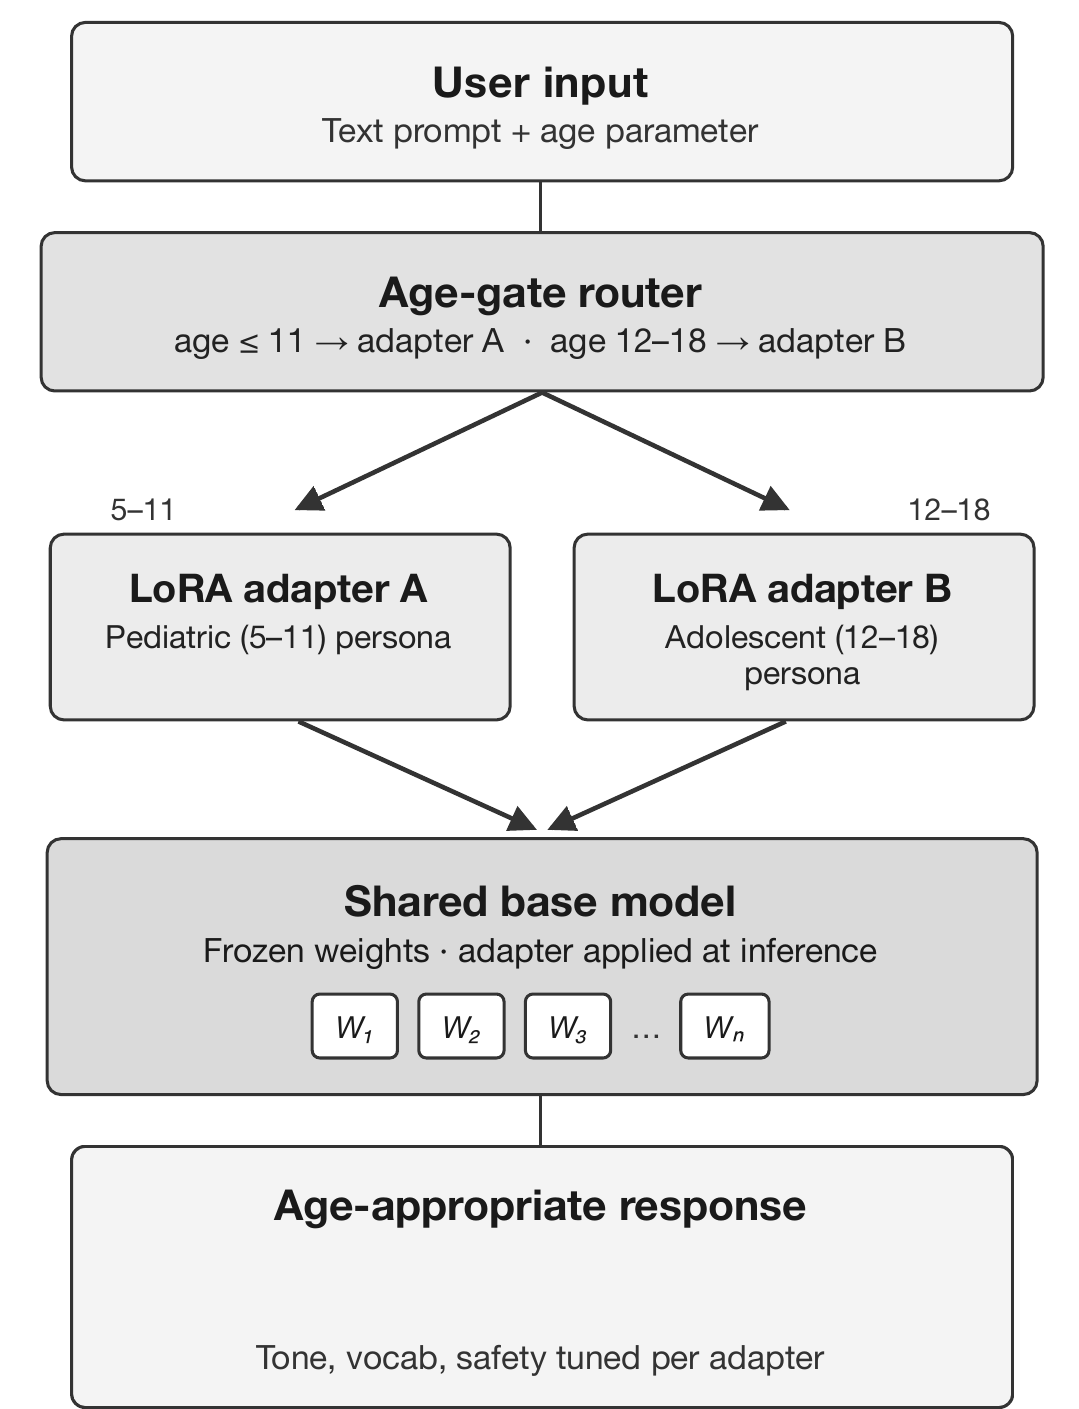
\includegraphics[width=0.85\linewidth]{images/architecture_diagram.png}
  \caption{Inference-time pipeline: \textit{guard-bear} gates raw user input before the age-gate router selects one of two LoRA adapters applied on top of the shared frozen base model. \textit{(Figure carried over from the prior submission and does not yet depict the guard-bear gating stage explicitly; see the note in the source file for a planned update.)}}
  \label{fig:architecture}
\end{figure}

\section{Data Generation Provenance}\label{secA3}

All response-model synthetic data was generated using Claude Opus 4.6 with extended thinking mode via Claude.ai Project Spaces (March 2026), with Victoria Hospital's publicly available patient and family guide attached as a grounding artifact in dedicated, per-category chats to maintain context isolation; the \texttt{edge\_cases} category was added in a later follow-up pass. Category definitions, per-category counts, and the hard safety rules enforced at generation time are given in Sections~\ref{subsec:responsedataset} and~\ref{sec:methodology}. \textit{guard-bear}'s dataset combines synthetic generation (safe and unsafe examples) with filtered examples pulled from existing public prompt-injection and jailbreak datasets, per Section~\ref{subsec:guarddataset}. Training scripts and evaluation code for both components were developed using Claude Code.

\section{Example Adapter Outputs}\label{secA4}

Table~\ref{tab:examples} shows representative responses from the Qwen 2.5-0.5B Fast configuration, one of the recommended deployment configurations (Section~\ref{sec:qwen25}), illustrating adapter behavior in the intended deployment context. Full validation-set outputs are available from the corresponding author upon request.

\begin{table*}[!h]
  \centering
  \caption{Example Qwen 2.5-0.5B Fast responses for both age groups.}
  \label{tab:examples}
  \small
  \begin{tabular}{@{}p{0.15\linewidth}p{0.37\linewidth}p{0.39\linewidth}@{}}
    \toprule
    Age / Cat. & Question & Response \\
    \midrule
    5--11, What to Expect &
    ``I'm walking around in here and I see a big room with lots of toys and games. What's that room for?'' &
    ``That's a hospital! The big room you're seeing is called the B1-B2 Unit. It has lots of special toys and games to help kids feel more comfortable while they're in the hospital. There are also crafts, puzzles, and board games for your family to play together too!'' \\
    5--11, Who Are These People? &
    ``I see a dog walking around with someone wearing a special vest. Is that dog allowed to be here?'' &
    ``That dog is a therapy animal, and it's really important to let them do their job. The special vest you see is called a therapy vest, and it's there to help the dog feel more comfortable. The hospital or animal shelter will make sure everything is ready for you to bring your dog inside, and they'll let the therapy volunteers know when it's okay.'' \\
    12--18, Emotional Reassurance &
    ``Looking around at all this before my actual visit is making my anxiety worse, not better.'' &
    ``That's a lot of stress. You're right, anxiety is real, and it can be hard to manage when you feel like your body's telling you something. But the hospital is a real place, and it might be worth going through this experience with you. You can talk to your care team about what they'd like and need from the visit, or ask for a distraction. You don't have to go through this alone, your care team can help you feel less anxious about the process.'' \\
    \bottomrule
  \end{tabular}
\end{table*}

\end{appendices}

\begin{thebibliography}{99}

\bibitem{zhou2023lima}
C.~Zhou, P.~Liu, P.~Xu, S.~Iyer, J.~Sun, R.~Maddela, X.~Peng, S.~Shrivastava, M.~Lewis, L.~Zettlemoyer, and O.~Levy, ``LIMA: Less Is More for Alignment,'' in \textit{Advances in Neural Information Processing Systems (NeurIPS)}, 2023.

\bibitem{dubey2024llama3}
A.~Dubey et al., ``The Llama 3 Herd of Models,'' \textit{arXiv preprint arXiv:2407.21783}, Meta AI, 2024.

\bibitem{apple2023mlx}
Apple, ``MLX: Efficient and Flexible Machine Learning on Apple Silicon,'' 2023. [Online]. Available: \url{https://github.com/ml-explore/mlx}

\bibitem{hu2022lora}
E.~J.~Hu, Y.~Shen, P.~Wallis, Z.~Allen-Zhu, Y.~Li, S.~Wang, L.~Wang, and W.~Chen, ``LoRA: Low-Rank Adaptation of Large Language Models,'' in \textit{Proc. Int. Conf. Learning Representations (ICLR)}, 2022.

\bibitem{kincaid1975fk}
J.~P.~Kincaid, R.~P.~Fishburne, R.~L.~Rogers, and B.~S.~Chissom, ``Derivation of New Readability Formulas for Navy Enlisted Personnel,'' Research Branch Report 8-75, Naval Technical Training Command, 1975.

\bibitem{mclaughlin1969smog}
G.~H.~McLaughlin, ``SMOG Grading --- A New Readability Formula,'' \textit{J. Reading}, vol.~12, no.~8, pp.~639--646, 1969.

\bibitem{gunning1952fog}
R.~Gunning, \textit{The Technique of Clear Writing}. New York, NY, USA: McGraw-Hill, 1952.

\bibitem{coleman1975cli}
M.~Coleman and T.~L.~Liau, ``A Computer Readability Formula Designed for Machine Scoring,'' \textit{J. Applied Psychology}, vol.~60, no.~2, pp.~283--284, 1975.

\bibitem{bansal2023textstat}
S.~Bansal, ``textstat: Python Library to Calculate Readability Statistics of a Text Object'' (v0.7.13), 2023. [Online]. Available: \url{https://pypi.org/project/textstat/}

\bibitem{dettmers2023qlora}
T.~Dettmers, A.~Pagnoni, A.~Holtzman, and L.~Zettlemoyer, ``QLoRA: Efficient Finetuning of Quantized LLMs,'' in \textit{Advances in Neural Information Processing Systems (NeurIPS)}, 2023.

\bibitem{biderman2024lora}
D.~Biderman, J.~G.~Ortiz, J.~Portes, M.~Paul, P.~Greengard, C.~Jennings, D.~King, S.~Havens, V.~Chiley, J.~Frankle, C.~Blakeney, and J.~P.~Cunningham, ``LoRA Learns Less and Forgets Less,'' \textit{Transactions on Machine Learning Research (TMLR)}, 2024.

\bibitem{pedregosa2011sklearn}
F.~Pedregosa et al., ``Scikit-learn: Machine Learning in Python,'' \textit{J. Machine Learning Research}, vol.~12, pp.~2825--2830, 2011.

\bibitem{allal2025smollm2}
L.~B. Allal et al., ``SmolLM2: When Smol Goes Big,'' \textit{arXiv preprint arXiv:2502.05737}, Hugging Face, 2025.

\bibitem{hospitalguide}
``Children's Hospital Patient and Family Guide,'' Children's Hospital London Health Sciences Centre. \url{https://www.lhsc.on.ca/childrens-hospital/childrens-hospital-patient-and-family-guide} (accessed Mar.\ 26, 2026).

\bibitem{promptguard2024}
Meta AI, ``Prompt-Guard-86M,'' 2024. [Online]. Available: \url{https://huggingface.co/meta-llama/Prompt-Guard-86M}

\bibitem{he2021deberta}
P.~He, X.~Liu, J.~Gao, and W.~Chen, ``DeBERTa: Decoding-enhanced BERT with Disentangled Attention,'' in \textit{Proc. Int. Conf. Learning Representations (ICLR)}, 2021.

\end{thebibliography}

\end{document}
